\label{chap:background}
This chapter is devoted to a discussion of our Target Exascale Architecture (TEA), and the challenges and opportunities for self-awareness within exascale architectures. The TEA is inspired by the Runnemede architecture used in the Traleika Glacier Extreme Scale software stack~\cite{Runnemede, IntelEAS}, and is representative of the organization of heterogeneous architectures for exascale computing. In practice, the TG software stack is used by Intel to simulate exascale-level many core chips.

%\section{Control Theoretic}
%%{
%    \textbf{\color{red} FIXME: Add basic information...}
%%}

\section{Target Exascale Architecture}
%{
    This section discusses various aspects of our TEA. These range from chip organization, to the envisioned toolchain. We end with a brief discussion of the challenges and opportunities within exascale architectures.
    \subsection{Chip Level Organization}
    %{
        \begin{figure}[htb!]
            \centering
            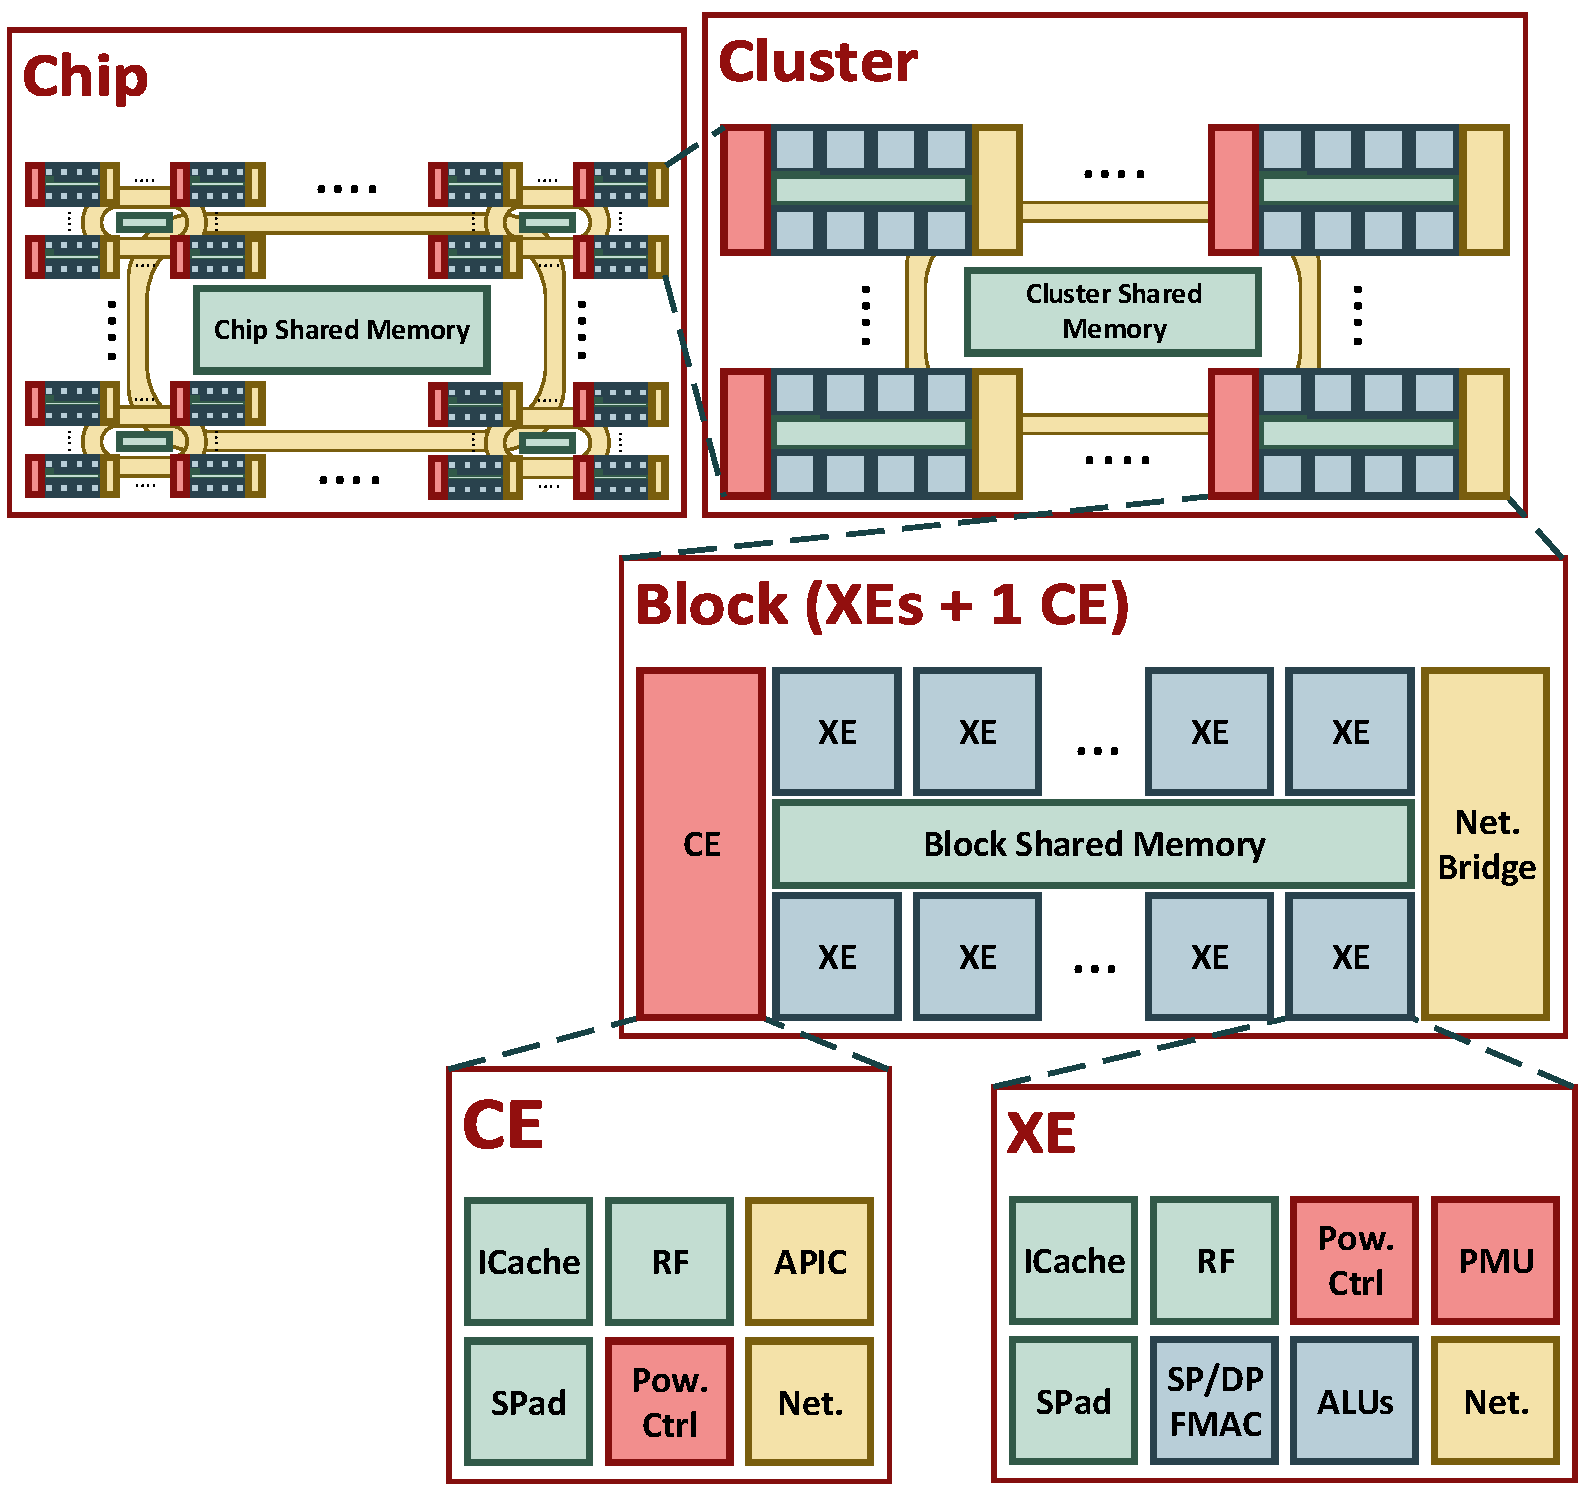
\includegraphics[width=0.9\textwidth]{Fig/TEA_architecture.pdf}
            \caption[Target Exascale Architecture]{Our Target Exascale Architecture consists of heterogeneous cores in a hierarchical configuration with network interconnects at each level, organized into blocks, clusters, and chips. Given the abstract nature of the architecture the exact number of cores and levels is not important and could vary. }
            \label{fig:TEA}
        \end{figure}

        At the lowest level, the TEA is organized into blocks consisting of a Control Engine (CE), several eXecution Engines (XEs), and a block shared memory. This organization is designed to decouple algorithmic workload from system monitoring and control. An XE's fundamental usage is to execute arbitrary code without interruption. The CE on the other hand is designed to control and schedule work to a number of local XEs within a given block, as well as, handle I/O negotiation, resource management, among other things. The overall abstract architecture is shown in Figure~\ref{fig:TEA}.
        
        Both XE and CE cores contain components commonly found in current architecture cores to support both data and code locality, such as, a register file (RF), instruction cache (ICache), and local memory which could be implemented as SPAD, a cache, or a hybrid. Additionally, they contain arithmetic and logic units (ALUs) and floating-point units (FPUs) of some form to support mathematical operations; however, the type of the support (e.g. vector processing) is abstracted away within the TEA. In a real architecture, it would be reasonable to assume that XEs and CEs are architecturally unique from one another in order to save die space and to facilitate the units to their primary role. As such, arithmetic support would likely be more limited in CEs than in XEs. It is worth noting that given the heterogeneous nature of the TEA, not all blocks must contain the same sets of hardware functionality. For example, some blocks could contain simpler XEs, and other blocks less but more complex XEs. 
        
        To enable fine-grained control over functional unit blocks (FUBs), clock and power gate control units are also provided. These function as knobs to control the state of individual FUBs in order to save power and energy, as well as, act as a fine-grained mechanism to manage on-chip temperatures. Furthermore, these serve to allow individual units to operate at near threshold voltage (NTV) within the system to minimize energy usage.
        
        To allow for individual blocks to be organized into a hierarchy, networking functionality is provided at the block level. The actual organization of this hierarchy in concrete terms, as well as, the on-chip networking hardware (e.g. bus, point-to-point, etc.) is abstracted away in the TEA. Furthermore, the TEA does not preclude the implementation of differing types of hardware at different levels of the hierarchy.

        Some distinct differences between XE and CE functionality include the addition of performance monitoring units (PMUs) within XE cores and an advanced programmable interrupt controller (APIC) within CE cores. Given that XEs are designed primarily for execution, the PMU provides a monitoring interface for use by the software stack running on-top of the TEA. Its use is to facilitate the collection of low-level metrics and enable high-level runtime decision making within the software stack using the said collected metrics. The APIC, on the other hand, facilitates CEs in the task of control by allowing interrupts and traps occurring within a block to be offloaded to the CE. Furthermore, any XEs requiring control type operations would generate interrupts to be serviced by the CE.
    %}

    \subsection{Target Exascale Architecture Toolchain}
    %{
        \begin{figure}[htb!]
            \centering
            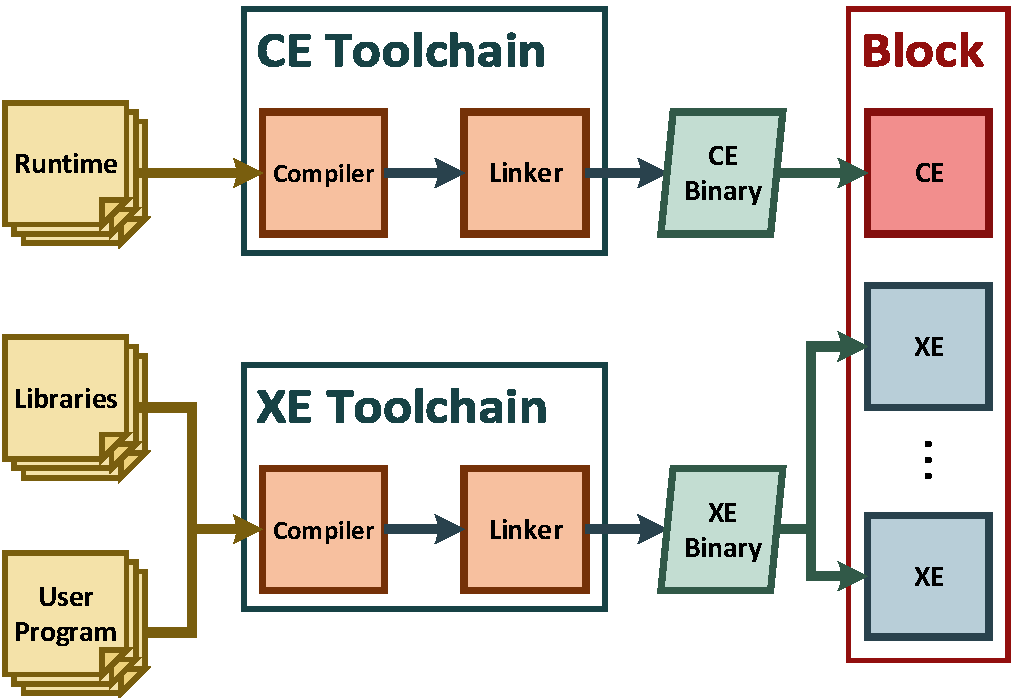
\includegraphics[width=0.7\textwidth]{Fig/TEA_toolchain.pdf}
            \caption[Target Exascale Architecture Toolchain]{An abstraction of a toolchain for the TEA. In such an architecture, CEs and XEs may be architecturally distinct allowing for separate toolchains. Shown above is one possible toolchain where the runtime system is compiled and linked using a separate toolchain from that of user programs.}
            \label{fig:TEA-toolchain}
        \end{figure}

        The TEA toolchain is shown in Figure~\ref{fig:TEA-toolchain}. In the TEA, XEs may be architecturally distinct from those of CEs and as a result a separate compiler and linker may be used to produce XE programs. As input, an XE would have basic library functionality compiled and linked to a user program. The CE, on the other, may use a completely separate set of libraries and features oriented toward its primary task. It is worth noting that given heterogeneous nature of the TEA that different blocks may be architecturally unique. As such, the TEA does not preclude separate toolchains for architecturally distinct blocks, and the example toolchain is only one possible toolchain that a real architecture implementing the TEA could use.
    %}
%}

\section{Challenges and Opportunities for Self-awareness}
%{
    There are number of challenges in the move toward exascale architectures. Energy becomes a primary and ever increasing issue because of the aforementioned multiplicity of components and transistors. Moreover, current execution paradigms will no longer suffice in terms of either performance, fault tolerance, and energy. Additionally, because communication and data accesses become prohibitively expensive between far memories and cores, this leads to the need for intelligent system software designed to minimize energy while also maximizing performance. Furthermore, this leads to the need for additional hardware mechanisms to enable system software to monitor system state efficiently and accurately. The details of which will be discussed in Chapter~\ref{chap:requirements}.

    Toward this end, current trends in high performance computing have been in developing fine-grained program execution models (PXMs) that limit data movement and allow for better control over resource usage in the presence of massively scale systems~\cite{KnauerhaseEtAl2012, OCR_SC12, TM104, ZuckermanEtAl2011, LauderdaleEtAl2012, SuetterleinZucGao2013}. These types of models are set to improve performance and reduce power consumption when combined with intelligence adaptive scheduling and resource management as discussed in my prior work~\cite{ZuckermanEtAl2014}. Additionally, the nature of these models in terms of self-contained explicit memory movement and code execution lends itself well to adaptive fault tolerance techniques. Some of my own prior work~\cite{KaplanEtAl2015} was on incorporating containment domains~\cite{Containment2012} into fine-grained PXMs to enable adaptive resilience within these types of models. Containment domains are a hierarchical scheme for creating robust data replication and task re-execution specifically geared toward exascale computing. Although, this thesis only touches upon resiliency in terms of hardware requirements, it is a fundamentally important challenge that needs to be explored for exascale architectures.
%}
